\documentclass{article}
\usepackage[T1]{fontenc}
\usepackage{lmodern}
\usepackage{graphicx}
\usepackage{amsmath,amssymb}
\usepackage[a4paper,margin=2cm]{geometry}
\usepackage[absolute,overlay]{textpos}
\setlength{\TPHorizModule}{1mm}
\setlength{\TPVertModule}{1mm}
\usepackage[indonesian]{babel}
\usepackage{hyperref}
\setlength{\emergencystretch}{2em}
% unit: Halaman 14

\begin{document}

% === Halaman 14 (llm) ===

\vspace{238.79mm}

\textbf{Tabel 1. Jumlah pergeseran bit pada setiap putaran}

\begin{tabular}{cc}
Putaran, $i$ & Jumlah pergeseran bit \\
\hline
1 & 1 \\
2 & 1 \\
3 & 2 \\
4 & 2 \\
5 & 2 \\
6 & 2 \\
7 & 2 \\
8 & 2 \\
9 & 1 \\
10 & 2 \\
11 & 2 \\
12 & 2 \\
13 & 2 \\
14 & 2 \\
15 & 2 \\
16 & 1 \\
\end{tabular}

% deskripsi: Diagram alir proses kriptografi yang menunjukkan langkah-langkah permutasi PC-1, pemisahan menjadi C dan D, operasi Left Shift berulang, dan permutasi PC-2 untuk menghasilkan kunci K1 hingga K16.
% bbox normalisasi: [0.0600, 0.1080, 0.9400, 0.9120]
\begin{textblock*}{184.80mm}(12.60mm,32.08mm)
\noindent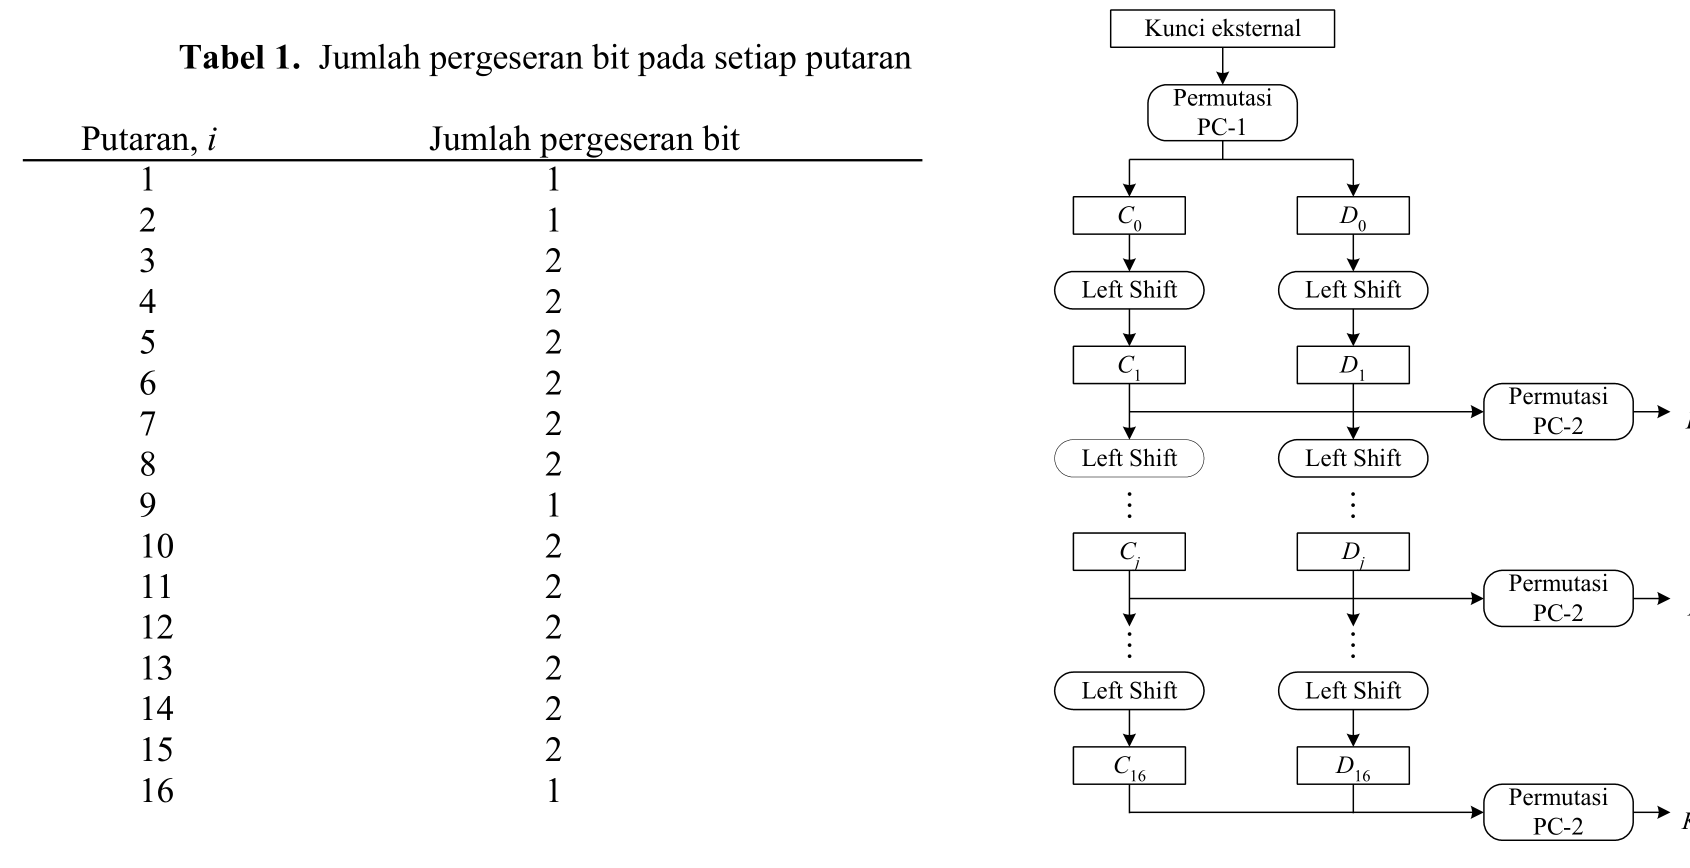
\includegraphics[width=184.80mm,height=238.79mm]{../../images/llm/page_014_img_01.png}%
\end{textblock*}

% bbox perkiraan otomatis: Diagram alir proses kriptografi yang menunjukkan langkah-langkah permutasi PC-1, pemisahan menjadi C dan D, operasi Left Shift berulang, dan permutasi PC-2 untuk menghasilkan kunci K1 hingga K16.

\end{document}
